
{
	\renewcommand{\secimage}{./media/aesthetics/S3}
	\section{Asymptotics on the Partition Function}
}

\begin{frame}{Quick recap}
	\vspace{0.1cm}
	\begin{columns}
		\begin{column}{0.5\textwidth}
			\only<1>{
			\vspace{-1cm}
			\begin{equation*}
				\dd \eP(\m{X}) = \prod_ {i < j}^n |z_i - z_j|^2 \prod_{j=i}^{n} \ee^{- n \Q(z_i)} \dd^2 z_i \dd \m{U}.
			\end{equation*}
			}
			\only<2-3>{
			\begin{equation*}
				p_n(\{z_i\}_{i=1}^n) = \frac{1}{\pZ{n}{Q}} \prod_ {i < j}^n |z_i - z_j|^2 \prod_{j=i}^{n} \ee^{- n \Q(z_i)} 
			\end{equation*}
			}
			\only<4-5>{
			\begin{align*}
					& p_n(\{z_i\}_{i=1}^n) = \frac{\ee^{-n^2 \Hf(\chi_n)}}{\pZ{n}{Q}}, \quad \text{with}\\
					& \Hf(\chi_n) = \frac{1}{n} \sum_{i = 1}^{n} \Q(z_i) + \frac{1}{n^2} \sum_{i \neq j}^{n} \ln |z_i - z_j|.
			\end{align*}
			}
			\only<6->{
				\begin{align*}
					& U^{\mu}(z) \deff \int \ln \frac{1}{|z - t|} \dd \mu(t), \\
					& I_Q(\mu) \deff \int U^{\mu}(s) \dd \mu(s) + \int \Q(s) \dd  \mu(s), \\
					& \mu_Q \quad \text{minimizer of $I_Q$}.
				\end{align*}
			}
		\end{column}
		\begin{column}{0.5\textwidth}
			\only<1-2>{
			\begin{table}
				\centering
				\begin{tabular}{l | c | c }
					$\eP(\m{X})$ & $\Se$ & $\M_n$ \\
					\hline \hline
					$\ee^{-n \tr(\m{M}^2)}$ &$\R$  & General\\ 
					$\ee^{-n \tr{(\m{X}^* \m{X})}}$ &  \cellcolor{red!10}$\C$ &  Hermitian \\
					\cellcolor{blue!10}$\ee^{-n \tr{(Q(\m{X}))}}$ & $\mathbb{H}$ & \cellcolor{green!10}Normal \\
					\vdots  & \vdots  &  \vdots \\
					\hline
					\multicolumn{3}{c}{	\fcolorbox{white}{blue!10}{} \!\!\!\! \fcolorbox{white}{red!10}{}  \!\!\!\! \fcolorbox{white}{green!10}{}} \\
					\multicolumn{3}{c}{Orthogonal Polynomial Ensemble} 
				\end{tabular}
			\end{table}
			}
			\only<3-4>{
				\begin{center}
					\begin{tikzpicture}[scale=0.90]
					\begin{axis}[axis line style={opacity=1}, ticks=none,
						xmin=-1.5, xmax=1.5,
						ymin=-1.5, ymax=1.5,
						axis x line=middle,
						axis y line=middle,
						xticklabel=\empty,
						yticklabel=\empty,
						xticklabel pos=top,
						xlabel=$\R$,
						ylabel=$\ii$,
						scatter/classes={%
							a={ mark size=0.5pt}}
						]
						\addplot[skip coords between index={100}{500}, opacity=1, scatter, mark=x, black, only marks] table [col sep=comma] {./media/aesthetics/5lines/a2t0.csv};
					\end{axis}
					\end{tikzpicture}
				\end{center}
			}
			\only<5->{
				\begin{center}
					\begin{tikzpicture}[scale=0.90]
						\begin{axis}[axis line style={opacity=1}, ticks=none,
							xmin=-1.5, xmax=1.5,
							ymin=-1.5, ymax=1.5,
							axis x line=middle,
							axis y line=middle,
							xticklabel=\empty,
							yticklabel=\empty,
							xticklabel pos=top,
							xlabel=$\R$,
							ylabel=$\ii$,
							scatter/classes={%
								a={ mark size=0.5pt}}
							]
							\addplot[opacity=0.07, scatter, mark=*,draw opacity=0,black, only marks] table [col sep=comma] {./media/aesthetics/5lines/a2t0.csv};
						\end{axis}
					\end{tikzpicture}
				\end{center}
			}
		\end{column}
	\end{columns}
	\visible<7->{
	\begin{align*}
			& p_n(\{z_i\}_{i=1}^n) = \frac{\ee^{-n^2 \Hf(\chi_n)}}{\pZ{n}{Q}}, \quad \text{with}\\
			& \Hf(\chi_n) = \frac{1}{n} \sum_{i = 1}^{n} \Q(z_i) + \frac{1}{n^2} \sum_{i \neq j}^{n} \ln |z_i - z_j|.
	\end{align*}
	\vspace{0.1cm}
	\visible<8>{
	\begin{equation*}
		\ln(\pZ{n}{Q}) = -I_Q n^2+\frac{1}{2} n\ln n+E_Q n+G\ln n+F_Q + o(1).
		\label{Equation: asymptotic for free energy}
	\end{equation*}
	}
	}
\end{frame}

\subsection{Sketch of Asymptotic Analysis}

\begin{frame}{Sketch}
	\begin{enumerate}
		\item \textit{Partition functions can be expressed in terms of the \textcolor{red}{norming constants}}:  We can write the free energy as
		\begin{equation*}
			\ln \pZ{n}{Q} = \ln{n!} + \sum_{j=0}^{n-1} \ln{h_j}.
		\end{equation*} \pause
		\item \textit{Asymptotics of norming constant using the asymptotic \textcolor{red}{Laplace technique}} .
		\begin{equation*}
			h_j = \int_{\C} |z|^{2j} \ee^{-n Q(z)} \dd^2 z \approx \frac{\ee^{-n V_{\tau(j)}(r_c(\tau(j)))}}{\sqrt{n}}.
		\end{equation*} \pause
		\item \textit{Asymptotic of the summation on $\ln h_j$ using \textcolor{red}{quadrature techniques}}: 
		\begin{equation*}
			- \sum_{j=0}^{n-1} \ln{h_j} \approx - n^2 \int_{r_0}^{r_1} V(r) \frac{(r q'(r))'}{2} \dd r = - n^2 I_Q[\mu_Q].
		\end{equation*}
	\end{enumerate}
\end{frame}

\subsection{Partition Function of Norming Constants}

\begin{frame}{Determinantal P.P.}
	\only<1-5>{
	\vspace{-1cm}
	}
 	Remember that the j.p.d.f. considered, with $\wf(z_i) = \ee^{-nQ(z_i)}$, is
	\begin{equation*}
		\only<1-4>{
			p_n(\mmany{z}{n}) = \frac{1}{\pZ{n}{Q}} \prod_ {i < j}^n |z_i - z_j|^2 \prod_{i=1}^{n} \wf(z_i)
		}
		\only<5-7>{
			p_n(\mmany{z}{n}) = \frac{\prod_{l=1}^{n} h_{n,l}}{\pZ{n}{Q}} \det\left[ K(z_i, z_j) \right]_{n\times n} 
		}
	\end{equation*}
	\only<1>{\vspace{2cm}}
	\only<1-5>{
		\vspace{0.5cm}
		
		\visible<2-5>{
			With $\prod_{i<j}^{n} |z_i - z_j| = {\det\left(q_{j-1}(z_i)\right)}_{n\times n}$ and $(\det(A))^2 = \det(\sum_{j=1}^{n} \overline{A_{ji}} A_{jk})$,
			\only<2>{
				\begin{equation*}
					\prod_{i<j}^{n} |z_i - z_j|^2 = \det\left(\sum_{l=1}^{n} \overline{q_{l-1,n}(z_i)} q_{l-1,n}(z_j) \right)_{n\times n}
				\end{equation*}
			}
			\only<3>{
				\begin{equation*}
					\frac{\prod_{i=1}^{n}\wf(z_i)}{\prod_{l=1}^{n} h_{n,l} }\prod_{i<j}^{n} |z_i - z_j|^2 = \det\left(\sqrt{\wf(z_i)\wf(z_j)}\sum_{l=1}^{n} \frac{1}{h_{k, n}} \overline{q_{l-1,n}(z_i)} q_{l-1,n}(z_j) \right)_{n\times n}
				\end{equation*}
			}
			\only<4->{
				\begin{equation*}
					\frac{\wf(z_i)}{\prod_{l=1}^{n} h_{n,l} } \prod_{i<j}^{n} |z_i - z_j|^2 = \det\left( K(z_i, z_j) \right)_{n\times n}
				\end{equation*}
			}
			where $q_i$ form a polynomial basis for the space.
		}
	}
	\only<6>{
		\vspace{-0.4cm}
		\begin{theorem}
			Let $\{q_{j,n}\}_{j=0}^\infty$ be a family of monic polynomials such that each $q_j(\lambda)$ is of degree $j$. Impose also that exists finite positive constants $\{h_{j,n}\}_{j=0}^\infty$ s.t.
			\begin{equation*}
				\langle q_{j,n}, q_{k,n} \rangle_{\wf} = \int_{\C} q_{j,n}(z) \overline{q_{k,n}(z)} \ee^{-nQ(z)} \dd^2 z = h_{j,n} \delta_{\{j=k\}}
			\end{equation*}	
			for any $j,k>0$. Then, $K_n(x,y)$ has reproducing properties, i.e.
			\begin{equation*}
				\int_{\C} \det\left[ K(\lambda_i, \lambda_j) \right]_{i,j=1}^{k+1} \dd^2 \lambda_{k+1} = (n-k) \det\left[ K(\lambda_i, \lambda_j) \right]_{i,j=1}^{k}.
			\end{equation*}
		\end{theorem}
	}
	\only<7>{
		\begin{colorblock}{Corollary}{bg=Mahogany,fg=white}
			Because of
			\begin{equation*}
				\int_{\C} \det\left[ K(\lambda_i, \lambda_j) \right]_{i,j=1}^{k+1} \dd^2 \lambda_{k+1} = (n-k) \det\left[ K(\lambda_i, \lambda_j) \right]_{i,j=1}^{k},
			\end{equation*}
			the partition function $\pZ{n}{Q}$ can be written as
			\begin{equation*}
				\pZ{n}{Q} = \prod_{l=1}^n h_{n,l}  \int_{\C^n} \det\left[ K(\lambda_i, \lambda_j) \right]_{i,j=1}^{n} \prod_{i=1}^{n} \dd^2 \lambda_i = n! \prod_{l=1}^n h_{n,l}
			\end{equation*}
		\end{colorblock}
	}
\end{frame}

\subsection{Asymptotic of Norming Constants}

\begin{frame}{Norming constants}
	\only<1-4>{
		We want to find
		\begin{equation*}
		\int_{\C} P_k(x) \overline{P}_m(x) \wf(x) \dd^2 z = \langle P_k, P_m \rangle_w = 
		\begin{cases}
			h_{n,m} & \text{if $m = k$}, \\
			0 & \text{if $m \neq k$}.
		\end{cases}
	\end{equation*} 
	\visible<2->{
	Notice that
	\begin{align*}
		\langle z^m , z^j \rangle_w & = \int_{\C} z^{m}\bar{z}^{j} \ee^{-n Q(z)} \dd^2 z, \\
		\visible<3->{
		& = \int_{0}^{\infty} \int_{0}^{2\pi} r^{m+j} \ee^{\ii \theta (m- j)} \ee^{-n q(r)} \frac{r}{\pi} \dd r \dd \theta, \\
		& = \frac{1}{\pi} \int_{0}^{2\pi} \ee^{\ii \theta (m - j)} \dd \theta \int_{0}^{\infty} r^{m+j+1} \ee^{-n q(r)} \dd r \\
		} \visible<4>{
		& = \begin{cases}
		 0, \quad \text{if} \  m \neq j, \\
		\int_{0}^{\infty} 2 r^{2j+1} \ee^{-n q(r)} \dd r, \quad \text{if} \  m = j. \\
		\end{cases}
		}
	\end{align*}
	}}
	\only<5->{
	Defining $z = r \ee^{\ii \theta}$ ($|z| = r$), \only<2->{because of the symmetry on $Q$ we write}
	\begin{align*}
		h_j & = \int_{\C} |z|^{2j} \ee^{-n Q(z)} \dd^2 z \\
		& = \int_{\Theta} \int_{\R_+} r^{2j} \ee^{-n q(r)} \frac{r}{\pi} \dd r \dd \theta, \\
		& = 2 \int_{\R_+} r^{2j+1} \ee^{-n q(r)} \dd r, \\
		& =  \int_{\R_+} 2 r \ee^{-n \left( q(r) - \frac{2j}{n} \ln(r) \right)} \dd r.
	\end{align*}
	\visible<6->{
	We redefine our potential using 
	\begin{equation*}
		V_{\tau(j)}(r) = q(r) - 2 \tau(j) \ln(r),
	\end{equation*}
	where $\tau(j) \deff j/n \in [0, 1)$. Then, rewrite the integral as
	\begin{equation*}
		h_j = \int_{\R_+} 2r \ee^{-n V_{\tau(j)}(r)} \dd r.
	\end{equation*}
	}
	}
\end{frame}

\begin{frame}
	Taking a look at the first derivative of the newly defined potential we find that the critical point $r_c$ must satisfy
	\begin{equation*}
		V'_\tau(r) = q'(r) - \frac{2\tau}{r} \quad \implies \quad r_c q'(r_c) = 2 \tau.
	\end{equation*}
	\visible<2->{
	Denote $r_{\tau(j)}$ the $r$ such that $ r q'(r) = 2 \tau(j)$. \visible<3->{Also define the limit points when $\tau = 0$ and $\tau = 1$ as
	\begin{equation*}
		\begin{cases}
			r_0, \quad \text{the largest solution of} \ r q'(r) = 0, \\
			r_ 1, \quad \text{the smallest solution of} \ r q'(r) = 2.
		\end{cases}
	\end{equation*}
	\begin{figure}[h!]
		\centering
		\hspace{1.1cm}
		\begin{subfigure}[t]{0.4\textwidth}
			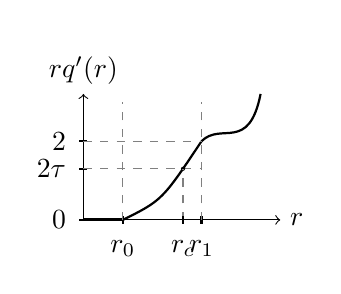
\begin{tikzpicture}[scale=0.5]
			\draw[->] (0,0) -- (5,0) node[right, label] {$r$};
			\draw[->] (0,0) -- (0,3.2) node[above, label] {$rq'(r)$};
			
			\draw[thick] (-0.1,0) -- (0.1,0) node[left=4pt, label] {$0$};
			\draw[thick] (-0.1,2) -- (0.1,2) node[left=4pt, label] {$2$};
			
			\draw[thick] (1,-0.1) -- (1,0.1) node[below=5pt, label] {$r_0$};
			\draw[thick] (3,-0.1) -- (3,0.1) node[below=5pt, label] {$r_1$};
			
			% Function: zero on [0,r0], strictly increasing on [r0,r1], increasing after r1
			\draw[smooth, thick] (0,0.01) -- (1,0.01);
			\draw[smooth, thick] (1,0)
			.. controls (2.0,0.5) .. (3,2);
			\draw[smooth, thick] (3,2)
			.. controls (3.5,2.5) and (4.2,1.7) .. (4.5,3.2);
			
			\draw[thick] (-0.1,1.3) -- (0.1,1.3) node[left=4pt, label] {$2\tau$};
			\draw[gray, dashed, thin] (0,1.3) -- (3,1.3);
			
			\draw[gray, dashed, thin] (1, 0) -- (1,3);
			\draw[gray, dashed, thin] (3,0) -- (3,3);
			\draw[gray, dashed, thin] (0,2) -- (3,2);
			
			\fill (2.53,1.3) circle (1.5pt) node {};
			\draw[gray, dashed, thin] (2.53, 0) -- (2.53,1.3);
			\draw[thick] (2.53,-0.1) -- (2.53,0.1) node[below=5pt, label] {$r_c$};
			\end{tikzpicture}
		\end{subfigure}
		\begin{subfigure}[t]{0.4\textwidth}
			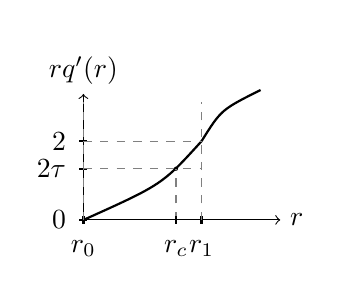
\begin{tikzpicture}[scale=0.5]
				\draw[->] (0,0) -- (5,0) node[right, label] {$r$};
				\draw[->] (0,0) -- (0,3.2) node[above, label] {$rq'(r)$};
				
				\draw[thick] (-0.1,0) -- (0.1,0) node[left=4pt, label] {$0$};
				\draw[thick] (-0.1,2) -- (0.1,2) node[left=4pt, label] {$2$};
				
				\draw[thick] (0,-0.1) -- (0,0.1) node[below=5pt, label] {$r_0$};
				\draw[thick] (3,-0.1) -- (3,0.1) node[below=5pt, label] {$r_1$};
				
				% Function: zero on [0,r0], strictly increasing on [r0,r1], increasing after r1
				\draw[smooth, thick] (0,0) -- (0,0);
				\draw[smooth, thick] (0,0)
				.. controls (2.0,0.9) .. (3,2);
				\draw[smooth, thick] (3,2)
				.. controls (3.5,2.8)  .. (4.5,3.3);
				
				\draw[thick] (-0.1,1.3) -- (0.1,1.3) node[left=4pt, label] {$2\tau$};
				\draw[gray, dashed, thin] (0,1.3) -- (3,1.3);
				
				\draw[gray, dashed, thin] (0, 0) -- (0,3);
				\draw[gray, dashed, thin] (3,0) -- (3,3);
				\draw[gray, dashed, thin] (0,2) -- (3,2);
				
				\fill (2.35,1.3) circle (1.5pt) node {};
				\draw[gray, dashed, thin] (2.35, 0) -- (2.35,1.3);
				\draw[thick] (2.35,-0.1) -- (2.35,0.1) node[below=5pt, label] {$r_c$};
			\end{tikzpicture}
		\end{subfigure}
	\end{figure}
	}}
\end{frame}

\begin{frame}
	\begin{equation*}
		h_j = \int_{\R_+} 2r \ee^{-n V_{\tau(j)}(r)} \dd r
	\end{equation*}
	\begin{figure}[h!]
		\centering
		\begin{tikzpicture}
			\begin{axis}[axis line style={opacity=1},
				width=\textwidth, height=6cm,
				legend style={draw=none},
				enlarge x limits = false,
				enlarge y limits = false,
				axis x line=bottom,
				axis y line=none,
				xtick={0},
				xticklabels = {$r^*$},
				xmin=-3,ymin=0,ymax=1.1,xmax=3
				]
				\path[name path=axis] (axis cs:-3,0) -- (axis cs:3,0);
				\only<1->{
				\addplot[name path=f1, domain=-3:3,smooth] {e^(-1*(cosh(x)-1))} ;
				\addplot [thick,color=black,fill=black, fill opacity=0.05] fill between[of=f1 and axis,soft clip={domain=-3:3}];
				}				\only<2->{
				\addplot[name path=f2, domain=-3:3,smooth] {e^(-2*(cosh(x)-1))} ;
				\addplot [thick,color=black,fill=black, fill opacity=0.05] fill between[of=f2 and axis,soft clip={domain=-3:3}];
				}				\only<3->{
				\addplot[name path=f3, domain=-3:3,smooth] {e^(-10*(cosh(x)-1)};
				\addplot [thick,color=black,fill=black, fill opacity=0.05] fill between[of=f3 and axis,soft clip={domain=-3:3}];
				}				\only<4->{
				\addplot[name path=f4, domain=-3:3,smooth] {e^(-70*(cosh(x)-1))};
				\addplot [thick,color=black,fill=black, fill opacity=0.05] fill between[of=f4 and axis,soft clip={domain=-3:3}];
				}
			\end{axis}
		\end{tikzpicture}
	\end{figure}
	\visible<5>{
		\begin{equation*}
		\lim_{n \rightarrow \infty} \frac{\ee^{-n(V_{\tau(j)}(r^*))}}{\ee^{-n(V_{\tau(j)}(r^* - \epsilon))}} = \lim_{n \rightarrow \infty} \ee^{-n(V_{\tau(j)}(r^*) - V_{\tau(j)}(r^* - \epsilon))} = \lim_{n \rightarrow \infty} \ee^{n |c|} \rightarrow + \infty. 
		\end{equation*}
	}
\end{frame}

\begin{frame}{Laplace Technique}
	We start by approximating $V_{\tau(j)}$ around its global minima by Taylor's theorem 
	\begin{equation*}
		V_{\tau(j)}(r) = V_{\tau(j)}(r^*) - \frac{1}{2} |V^{(2)}_{\tau(j)}(r^*)|(r-r^*)^2 + \epsilon((r-r^*)^3)
	\end{equation*}
	and then perform a change of variables $\frac{r}{\sqrt{n}} = s - r^*$, \pause so that 
	\begin{equation*}
	\!\!	\int_{r^*-\frac{\ln(n)}{\sqrt{n}}}^{r^*+\frac{\ln(n)}{\sqrt{n}}} 2s \ee^{-n V_{\tau(j)}(s)} \dd s \approx \frac{\ee^{-n  V_{\tau(j)}(r^*)}}{\sqrt{n}} \int_{-\ln(n)}^{\ln(n)} 2 \left(r^* + \frac{r}{\sqrt{n}}\right) \ee^{-\frac{1}{2} |V^{(2)}_{\tau(j)}(r^*)|r^2} \dd r
	\end{equation*}
	and
	\begin{equation*}
	\!\!	\int_{r^*+ \frac{\ln(n)}{\sqrt{n}}}^{\infty} |2s| \ee^{-n V_{\tau(j)}(s)} \dd(s) \leq \ee^{-n V_{\tau(j)}(r^*)} \epsilon_n
	\end{equation*}
\end{frame}

\begin{frame}
	\begin{theorem}
	(Laplace's Method) Let $\Phi$ be
	\begin{equation*}
		\Phi(n) = \int_{a}^{b} g(t) \ee^{-n \phi(t)} \dd t
			\label{equation: Laplace}
	\end{equation*}
	where $g(t) \ee^{-n \phi(t)}$ is absolutely integrable over $[a,b]$ for every $n$, the function $\phi(t)$ attains its maximum only at the point $c$ in $(a, b)$, the second derivative $\phi''(t)$ exists in a neighborhood of and is negative on $c$. Finally, $g(t)$ is non-zero and continuous at $c$. Then the function $\Phi$ satisfies an estimate of the form
	\begin{equation*}
		\Phi(n) = \ee^{-n \phi(c)} \left( \frac{\sqrt{2\pi} g(c)}{\sqrt{|\phi''(c)|}n^{1/2}} + \Boh(n^{-3/2})\right)
	\end{equation*}
	as $n \rightarrow \infty$.
	\end{theorem}
\end{frame}

\begin{frame}
	\begin{colorblock}{Theorem}{bg=Mahogany,fg=white}
	We have the following asymptotic of $n$ for $h_j$, with $0 \leq j \leq n-1$,
	\begin{equation*}
		h_j = \frac{\ee^{-n V_{\tau(j)}(r_{\tau(j)})}}{\sqrt{n}} \left( \frac{8\pi r_{\tau(j)}^2}{V^{(2)}_{\tau(j)}(r_{\tau(j)})} \right)^{\frac{1}{2}} \left[ 1 + \frac{1}{n} \mathfrak{B}(r_{\tau(j)}) + \Boh(n^{-2}) \right],
		\label{Equation: Asymptotic hj annulus}
	\end{equation*}
	where we have set 
	\begin{equation*}
		\mathfrak{B}(r_{\tau(j)}) \deff -\frac{V^{(4)}_{\tau(j)}(r_{\tau(j)})}{V^{(2)}_{\tau(j)}(r_{\tau(j)})^2} \frac{1}{8} - \frac{V^{(3)}_{\tau(j)}(r_{\tau(j)})}{V^{(2)}_{\tau(j)}(r_{\tau(j)})^{2}} \frac{1}{2 r_{\tau(j)}} - \frac{V^{(3)}_{\tau(j)}(r_{\tau(j)})^2}{V^{(2)}_{\tau(j)}(r_{\tau(j)})^{3}} \frac{5}{24}.
	\end{equation*}
	\end{colorblock}
\end{frame}

\subsection{Asymptotic of the Summation}


\begin{frame}{Quadrature}
	We have
	\begin{equation*}
		\ln \pZ{n}{Q} = \ln{n!} + \sum_{j=0}^{n-1} \ln{h_j}.
	\end{equation*}
	where
	\begin{equation*}
		h_j = \int_{\C} |z|^{2j} \ee^{-n Q(z)} \dd^2 z \approx \frac{\ee^{-n V_{\tau(j)}(r_c(\tau(j)))}}{\sqrt{n}}.
	\end{equation*}
	\visible<2->{
	\begin{columns}
		\begin{column}{0.4\textwidth}
			\begin{equation*}
				\Delta_n \sum_{j=0}^{n-1} \ln{h_j} \approx \int_{a}^{b} \ln{h_j}
			\end{equation*}
		\end{column}
		\begin{column}{0.6\textwidth}
			\vspace{-0.5cm}
				\begin{center}
				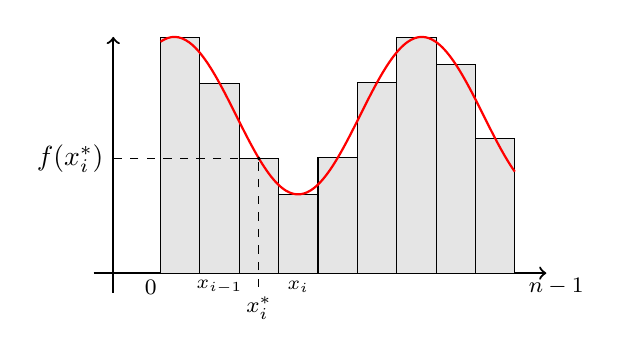
\begin{tikzpicture}[scale=0.5]
					\def\a{1.45}
					\def\b{9.75}
					\def\c{3.7}
%					\only<1-2>{
						\def\L{1} % width of interval
%					}
%					\only<3>{
%						\def\L{0.25} % width of interval
%					}
					\pgfmathsetmacro{\Va}{2*sin(\a r+1)+4} \pgfmathresult
					\pgfmathsetmacro{\Vb}{2*sin(\b r+1)+4} \pgfmathresult
					\pgfmathsetmacro{\Vc}{2*sin(\c r+1)+4} \pgfmathresult
					\draw[->,thick] (-0.5,0) -- (11,0) coordinate (x axis) node[below] {};
					\draw[->,thick] (0,-0.5) -- (0,6) coordinate (y axis) node[left] {};
%					\only<1-2>{
					\foreach \f in {1.7,2.7,...,9.7} {\pgfmathparse{2*sin(\f r+1)+4} 
%					}
%					\only<3>{
%					\foreach \f in {1.7,1.95,2.2,...,9.2} {\pgfmathparse{2*sin(\f r+1)+4} 
%					}
					\pgfmathresult
						\draw[fill=black!10] (\f-\L/2,\pgfmathresult |- x axis) -- (\f-\L/2,\pgfmathresult) -- (\f+\L/2,\pgfmathresult) -- (\f+\L/2,\pgfmathresult |- x axis) -- cycle;}
					\node at (\a-\L/2,-10pt) {\footnotesize{$0$}};
					\node at (\b+\L/2+\L,-10pt) {\footnotesize{$n -1$}};
					\draw[black] (\c-\L/2,0) -- (\c-\L/2,\Vc) -- (\c+\L/2,\Vc) -- (\c+\L/2,0);
					\draw[dashed] (\c,-10pt) node[below] {\footnotesize{$x^*_i$}} -- (\c,\Vc) -- (0,\Vc) node[left] {$f(x^*_i)$};
					\node at (\c-\L,-10pt) {\scriptsize{$x_{i-1}$}};
					\node at (\c+\L,-10pt) {\scriptsize{$x_i$}};
					%\node at (\a+5*\L,-5pt) {\footnotesize{$x_{i+1}$}};
					\draw[red,thick,smooth,samples=100,domain=1.2:10.2] plot(\x,{2*sin(\x r+1)+4});
					\filldraw[black] (\c,\Vc) circle (.03cm);
				\end{tikzpicture}
			\end{center}
		\end{column}
	\end{columns}
}
\end{frame}

\begin{frame}[allowframebreaks, allowdisplaybreaks]{Quadrature}
%	Following the computations in \citeonline{Trapezoidal-Maclaurin}, take a function $f \in C^p(\R)$ for $p \geq 1$. To derive the Euler-Maclaurin for the interval $[a,b]$, let $h = (b - a)/n$ and $c = a + j h$, then we express
%	\begin{equation}
%		\int_{a}^{b} f(x) \dd x = \sum_{j=0}^{n-1} \int_{a+j h}^{a+(j+1)h} f(x) \dd x
%	\end{equation}
%	where we use \eqref{Equation: Differential Bernoulli} and integration by parts to rewrite each integral as
%	\begin{align}
%		\int_{c}^{c+h} f(x) \dd x & = h \int_{0}^{1} B_0(1-x) f(c+xh) \dd x \\
%		& = - h \frac{B_1(1-x)}{1!} f(c + xh) |_0^1 + h^2 \int_{0}^{1} \frac{B_1(1-x)}{1!} f'(c+xh) \dd x, \\
%		& \vdots \nonumber \\
%		& = - \sum_{r = 0}^{p-1} \frac{h^{r+1} B_{r+1}(1-x)}{(r+1)!} f^{(r)}(c+xh) |_0^1 + h^{p+1} \int_0^1 \frac{h^{r+1} B_{p}(1-x)}{(p)!} f^{(p)}(c+xh) \dd x, \\
%		& 
%		\begin{multlined}
%			= h \frac{f(c) + f(c+h)}{2} - \sum_{r = 0}^{p-1} \frac{h^{r+1} B_{r+1}(1-x)}{(r+1)!} \left[ f^{(r)}(c+h) - f^{(r)}(c) \right] \\
%			+ h^{p+1} \int_0^1 \frac{B_{p}(1-x)}{(p)!} f^{(p)}(c+xh) \dd x. 
%		\end{multlined}
%	\end{align}
%	where one can start to notice, for instance, the trapezoidal rule creeping out on the first term. Notice that it was necessary to use that $ - B_1(0) = B_1(1) = 1/2$ and $B_n(0) = B_n(1) = B_n$ for $n\neq1$. 
We begin with $h  = (b - a)/n$, s.t.
\begin{align*}
	\int_{a}^{b} f(x) \dd x & \approx h \sum_{j = 0}^{n} f(x_j^*), \\
	& = h \sum_{j = 0}^{n} \frac{f(x_{j}) + f(x_{j-1})}{2}, \\
	& = h \left[ \frac{f(a)}{2} + f(a+h) + \cdots + f(b-h) + \frac{f(b)}{2} \right], \\
	& = h \sum_{j = 1}^{n-1} f(x_j^*) + \frac{h}{2} \left( f(b) + f(a) \right), \\
	& = h \sum_{j = 0}^{n-1} f(x_j^*) + \frac{h}{2} \left( f(b) - f(a) \right).
\end{align*}
\end{frame}

\begin{frame}
	\begin{theorem} (Euler-Maclaurin Formula)
		If $m$ and $n$ are natural numbers and $f(x)$ is a real or complex valued continuous function for real numbers $x$ in the interval $[m,n]$, then the integral can be approximated by the sum (or vice versa) 
		\begin{multline*}
			\! \! \! \! \! \sum_{i=m+1}^{n} f(i) = \int_{m}^{n} f(x) \dd x + \frac{f(n) - f(m)}{2} + \sum_{k=1}^{\lfloor \frac{p}{2} \rfloor} \frac{B_{2k}}{(2k)!} \left( f^{(2k-1)}(n) - f^{(2k-1)}(m)\right) +  R_p
		\end{multline*}
	\end{theorem}
		\begin{center}
		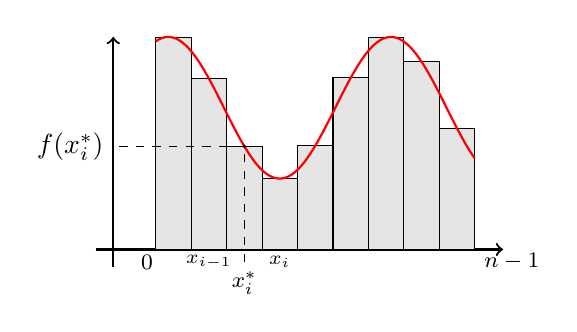
\begin{tikzpicture}[scale=0.45]
			\def\a{1.45}
			\def\b{9.75}
			\def\c{3.7}
			%					\only<1-2>{
				\def\L{1} % width of interval
				%					}
			%					\only<3>{
				%						\def\L{0.25} % width of interval
				%					}
			\pgfmathsetmacro{\Va}{2*sin(\a r+1)+4} \pgfmathresult
			\pgfmathsetmacro{\Vb}{2*sin(\b r+1)+4} \pgfmathresult
			\pgfmathsetmacro{\Vc}{2*sin(\c r+1)+4} \pgfmathresult
			\draw[->,thick] (-0.5,0) -- (11,0) coordinate (x axis) node[below] {};
			\draw[->,thick] (0,-0.5) -- (0,6) coordinate (y axis) node[left] {};
			%					\only<1-2>{
				\foreach \f in {1.7,2.7,...,9.7} {\pgfmathparse{2*sin(\f r+1)+4} 
					%					}
				%					\only<3>{
					%					\foreach \f in {1.7,1.95,2.2,...,9.2} {\pgfmathparse{2*sin(\f r+1)+4} 
						%					}
					\pgfmathresult
					\draw[fill=black!10] (\f-\L/2,\pgfmathresult |- x axis) -- (\f-\L/2,\pgfmathresult) -- (\f+\L/2,\pgfmathresult) -- (\f+\L/2,\pgfmathresult |- x axis) -- cycle;}
				\node at (\a-\L/2,-10pt) {\footnotesize{$0$}};
				\node at (\b+\L/2+\L,-10pt) {\footnotesize{$n -1$}};
				\draw[black] (\c-\L/2,0) -- (\c-\L/2,\Vc) -- (\c+\L/2,\Vc) -- (\c+\L/2,0);
				\draw[dashed] (\c,-10pt) node[below] {\footnotesize{$x^*_i$}} -- (\c,\Vc) -- (0,\Vc) node[left] {$f(x^*_i)$};
				\node at (\c-\L,-10pt) {\scriptsize{$x_{i-1}$}};
				\node at (\c+\L,-10pt) {\scriptsize{$x_i$}};
				%\node at (\a+5*\L,-5pt) {\footnotesize{$x_{i+1}$}};
				\draw[red,thick,smooth,samples=100,domain=1.2:10.2] plot(\x,{2*sin(\x r+1)+4});
				\filldraw[black] (\c,\Vc) circle (.03cm);
			\end{tikzpicture}
		\end{center}
\end{frame}

\begin{frame}
	We return to $\sum_{j=0}^{n-1} \ln{h_j}$ using the previous asymptotic
	\scriptsize
	\only<1>{
	\begin{equation*}
		= \sum_{j=0}^{n-1} \ln\left[ \frac{\ee^{-n V_{\tau(j)}(r_{\tau(j)})}}{\sqrt{n}} \left( \frac{8\pi r_{\tau(j)}^2}{V^{(2)}_{\tau(j)}(r_{\tau(j)})} \right)^{\frac{1}{2}} \left[ 1 + \frac{1}{n} \mathfrak{B}(r_{\tau(j)}) + \Boh(n^{-2}) \right] \right], 
	\end{equation*}
	}
	\only<2-3>{
	\begin{equation*}
		= \sum_{j=0}^{n-1} \left[-n V_{\tau(j)}(r_{\tau(j)}) + \frac{1}{2} \left(\ln(2\pi r^2_{\tau(j)}) - \ln n - \ln\left(\frac{V^{(2)}_{\tau(j)}(r_{\tau(j)})}{4}\right)  \right) + \frac{1}{n} \mathfrak{B}(r_{\tau(j)}) + \Boh(n^{-2})\right]
	\end{equation*}
	}
	\only<4-5>{
	\begin{multline*}
		= - n^2 I_Q[\mu_Q] + n U_{\mu_Q}(0) - 	\frac{1}{6} \ln{\left( \frac{r_0}{r_1}\right)} \\ + \sum_{j=0}^{n-1} \left[\frac{1}{2} \left(\ln(2\pi r^2_{\tau(j)}) - \ln n - \ln\left(\frac{V^{(2)}_{\tau(j)}(r_{\tau(j)})}{4}\right)  \right) + \frac{1}{n} \mathfrak{B}(r_{\tau(j)}) + \Boh(n^{-2})\right]
%		\sum_{j=0}^{n-1} \ln{h_j} = - n^2 I_Q[\mu_Q] + n U_{\mu_Q}(0) - \frac{1}{6} \ln{\left( \frac{r_0}{r_1}\right)}  - \frac{n}{2} \ln(n) - \frac{1}{2}  \left( n E_Q[\mu_Q] -  \frac{1}{2} \ln \left( \frac{V^{(2)}_{1}(r_1)}{V^{(2)}_{0}(r_{0})} \right) \right)	\\ + \frac{1}{2} \left( n \ln(2\pi) + 2 \left( - n U_{\mu_Q}(0) - \frac{1}{2} \ln\left(\frac{r_1}{r_0}\right) \right) \right)
%		- \frac{3}{32} \ln\left( \frac{V^{(2)}_1(r_1)}{V^{(2)}_0(r_0)} \right) \\ - \frac{1}{32} \left( \frac{r_1  V^{(3)}_1(r_1)}{V^{(2)}_1(r_1)} - \frac{r_0 V^{(3)}_0(r_0)}{V^{(2)}_0(r_0)}\right) - \frac{1}{12} \int_{r_0}^{r_1} \frac{V^{(3)}(r)^2}{V^{(2)}(r)^{2}} r \dd r +  \Boh(n^{-1})
	\end{multline*}
	}
	\only<6>{
		\begin{multline*}
			\sum_{j=0}^{n-1} \ln{h_j} = - n^2 I_Q[\mu_Q] + n U_{\mu_Q}(0) - \frac{1}{6} \ln{\left( \frac{r_0}{r_1}\right)}  - \frac{n}{2} \ln(n) - \frac{1}{2}  \left( n E_Q[\mu_Q] -  \frac{1}{2} \ln \left( \frac{V^{(2)}_{1}(r_1)}{V^{(2)}_{0}(r_{0})} \right) \right)	\\ + \frac{1}{2} \left( n \ln(2\pi) + 2 \left( - n U_{\mu_Q}(0) - \frac{1}{2} \ln\left(\frac{r_1}{r_0}\right) \right) \right) + \frac{1}{4} \int_{0}^{r_1} \mathfrak{B}(s) s V^{(2)}(s) \dd s + \Boh(n^{-1})
		\end{multline*}
	}
	\only<7->{
	\begin{multline*}
		\sum_{j=0}^{n-1} \ln{h_j} = - n^2 I_Q[\mu_Q] - \frac{n}{2} \ln(n) + n \left(\frac{\ln(2\pi)}{2} - \frac{1}{2} E_Q[\mu_Q]\right) - \frac{2}{3}  \ln{\left( \frac{r_0}{r_1}\right)}  + \frac{5}{32} \ln \left( \frac{V^{(2)}_{1}(r_1)}{V^{(2)}_{0}(r_{0})} \right) \\ - \frac{1}{32} \left( \frac{r_1  V^{(3)}_1(r_1)}{V^{(2)}_1(r_1)} - \frac{r_0 V^{(3)}_0(r_0)}{V^{(2)}_0(r_0)}\right) - \frac{1}{12} \int_{r_0}^{r_1} \frac{V^{(3)}(r)^2}{V^{(2)}(r)^{2}} r \dd r +  \Boh(n^{-1}).
	\end{multline*}
	}
	\only<1-2>{\vspace{5cm}}
	\only<4,6,7>{\vspace{4.5cm}}
	\normalsize
	\only<3>{
	\begin{colorblock}{Theorem}{bg=Mahogany,fg=white}
		\small
		\begin{equation*}
			- n \sum_{j=0}^{n-1} V_{\tau(j)}(r_{\tau(j)}) = - n^2 I_Q[\mu_Q] + n U_{\mu_Q}(0) - 	\frac{1}{6} \ln{\left( \frac{r_0}{r_1}\right)} + \Boh(n^{-2}), 
			\label{Equation: sum V annulus}
		\end{equation*}
		\normalsize
		where
		\small
		\begin{align*}
			&I_Q[\mu_Q] \deff \left[\frac{1}{4} \int_{r_0}^{r_1} q(s) s V^{(2)}(s) \dd s- \ln(r_1) + \frac{1}{2} q(r_1) \right],\\
			& - 2 U_{\mu_Q}(0) \deff \int_{r_0}^{r_1} \ln(s) (s q'(s))' \dd s  = q(r_1) - q(r_0) + 2 \ln(r_1).
		\end{align*}
		\normalsize
	\end{colorblock}
	}
	\only<5>{
		\begin{colorblock}{Theorem}{bg=Mahogany,fg=white}
			Asymptotically on $n$,
			\scriptsize
			\begin{align*}
				&\sum_{j=0}^{n-1}  \ln V^{(2)}_{\tau(j)}(r_{\tau(j)})  = n E_Q[\mu_Q] -   \frac{1}{2} \ln \left( \frac{V^{(2)}_{1}(r_1)}{V^{(2)}_{0}(r_{0})} \right) + \Boh(n^{-1}), \\
				&\sum_{j=0}^{n-1}  \ln(2\pi r^2_{\tau(j)}) = n \ln(2\pi) + 2 \left( - n U_{\mu_Q}(0) - \frac{1}{2} \ln\left(\frac{r_1}{r_0}\right) + \Boh(n^{-1}) \right), \\
				&\frac{1}{n} \sum_{j=0}^{n-1} \mathfrak{B}(r_{\tau(j)}) = \frac{1}{4} \int_{0}^{r_1} \mathfrak{B}(s) s V^{(2)}(s) \dd s + \Boh(n^{-2})
			\end{align*}
			where
			\begin{equation*}
				E_Q[\mu_Q] \deff \frac{1}{2} \int_{r_0}^{r_1} \ln\left(\frac{V^{(2)}(s)}{4}\right) (sq'(s))' \dd s.
			\end{equation*}
			\normalsize
		\end{colorblock}
	}
	\only<8>{
		\begin{colorblock}{Theorem}{bg=Mahogany,fg=white}
			Asymptotically on $n$,
			\small
			\begin{equation*}
				\sum_{j=0}^{n-1} \ln{h_j} = - n^2 I_Q[\mu_Q] - \frac{n}{2} \ln n + n \left(\frac{\ln(2\pi)}{2} - \frac{1}{2} E_Q[\mu_Q]\right) + F_V[A_{[r_0, r_1]}] + \Boh(n^{-1}) 
			\end{equation*}
			\normalsize
			where
			\scriptsize
			\begin{multline*}
				F_V[A_{[r_0, r_1]}]  \deff - \frac{2}{3} \ln\left(\frac{r_1}{r_0} \right) + \frac{5}{32} \ln\left( \frac{V^{(2)}_1(r_1)}{V^{(2)}_0(r_0)} \right) - \frac{1}{32} \left( \frac{r_1  V^{(3)}_1(r_1)}{V^{(2)}_1(r_1)} - \frac{r_0 V^{(3)}_0(r_0)}{V^{(2)}_0(r_0)}\right) - \frac{1}{12} \int_{r_0}^{r_1} \frac{V^{(3)}(r)^2}{V^{(2)}(r)^{2}} r \dd r,
			\end{multline*}
			\normalsize
		\end{colorblock}
	}
\end{frame}

\subsection{Final results}

\begin{frame}
	\only<1>{
	\begin{colorblock}{Theorem}{bg=Mahogany,fg=white}	\label{Theorem: Annulus Free Energy}
		For the annulus case, where $r_0 > 0$, we have the following expression for the free energy asymptotically on $n$ given by
		\scriptsize
		\begin{multline*}
			\ln{\pZ{n}{Q}} = - n^2 I_Q[\mu_Q] + \frac{n}{2} \left( \ln(2\pi) - E_Q[\mu_Q] - 2\right) + \frac{n}{2} \ln(n) + \frac{\ln(2\pi)}{2} + \frac{1}{2} \ln(n)+ F_V[A_{[r_0, r_1]}] + \Boh(n^{-1})        
		\end{multline*}
		\normalsize
		where
		\scriptsize
		\begin{equation*}
			I_Q[\mu_Q] \deff \left[\frac{1}{4} \int_{r_0}^{r_1} q(s) s V^{(2)}(s) \dd s- \ln(r_1) + \frac{1}{2} q(r_1) \right],
		\end{equation*}
		\begin{equation*}
			E_Q[\mu_Q] \deff \frac{1}{2} \int_{r_0}^{r_1} \ln\left(\frac{V^{(2)}(s)}{4}\right) (sq'(s))' \dd s.
		\end{equation*}
		\begin{multline*}
			F_V[A_{[r_0, r_1]}]  \deff - \frac{2}{3} \ln\left(\frac{r_1}{r_0} \right) + \frac{5}{32} \ln\left( \frac{V^{(2)}_1(r_1)}{V^{(2)}_0(r_0)} \right) - \frac{1}{32} \left( \frac{r_1  V^{(3)}_1(r_1)}{V^{(2)}_1(r_1)} - \frac{r_0 V^{(3)}_0(r_0)}{V^{(2)}_0(r_0)}\right) - \frac{1}{12} \int_{r_0}^{r_1} \frac{V^{(3)}(r)^2}{V^{(2)}(r)^{2}} r \dd r,
		\end{multline*}
		\normalsize
	\end{colorblock}
	}
	\only<2>{
	\begin{figure}[h!]
		\begin{subfigure}[t]{0.45\textwidth}
			\centering
			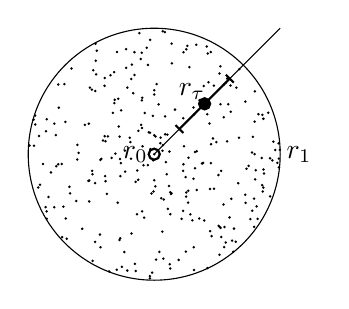
\begin{tikzpicture}[scale=0.8]
				% circles and line
				\draw (0,0) circle (2);
				\draw (0,0) -- (2,2);
				\node[thick] at (0,0) {\pgfuseplotmark{o}};
				%markings fro interval
				\draw[thick] (0.4,0.4) -- (1.2,1.2);
				\node[rotate=45, thick] at (0.4,0.4) {\pgfuseplotmark{|}};
				\node[rotate=45, thick] at (1.2,1.2) {\pgfuseplotmark{|}};
				\node[thick] at (0.8,0.8) {\pgfuseplotmark{*}};
				% labels
				\node at (0.6,1.0) {$r_\tau$};
				\node at (-0.3,0) {$r_0$};
				\node at (2.3,0) {$r_1$};
				% random points
				\foreach \x in {1,...,300}{
					\pgfmathsetmacro{\r}{sqrt(random(0,400)/100)}%
					\pgfmathsetmacro{\a}{random(0,360)}%
					\pgfmathsetmacro{\x}{\r*sin(\a)}
					\pgfmathsetmacro{\y}{\r*cos(\a)}
					\node[fill,circle,inner sep=0pt,minimum size=1pt] at (\x ,\y) {};
				}
			\end{tikzpicture}
		\end{subfigure}
		\begin{subfigure}[t]{0.45\textwidth}
			\centering
			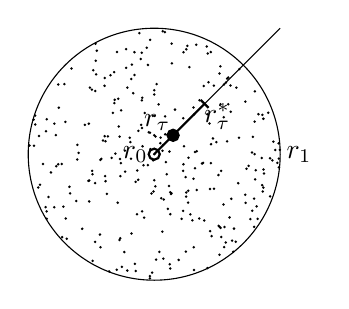
\begin{tikzpicture}[scale=0.8]
				% circles and line
				\draw (0,0) circle (2);
				\draw (0,0) -- (2,2);
				\node[thick] at (0,0) {\pgfuseplotmark{o}};
				%markings fro interval
				\draw[thick] (0.0,0.0) -- (0.8,0.8);
				\node[rotate=45, thick] at (0.8,0.8) {\pgfuseplotmark{|}};
				\node[thick] at (0.3,0.3) {\pgfuseplotmark{*}};
				% labels
				\node at (0.05,0.5) {$r_\tau$};
				\node at (-0.3,0) {$r_0$};
				\node at (2.3,0) {$r_1$};
				\node at (1.0,0.6) {$r_\tau^*$};
				% random points
				\foreach \x in {1,...,300}{
					\pgfmathsetmacro{\r}{sqrt(random(0,400)/100)}%
					\pgfmathsetmacro{\a}{random(0,360)}%
					\pgfmathsetmacro{\x}{\r*sin(\a)}
					\pgfmathsetmacro{\y}{\r*cos(\a)}
					\node[fill,circle,inner sep=0pt,minimum size=1pt] at (\x ,\y) {};
				}
			\end{tikzpicture}
		\end{subfigure}
	\end{figure}
	}
	\only<3>{
	\begin{colorblock} {Theorem}{bg=Mahogany,fg=white}	\label{Theorem: Disk Free Energy}
		For the disk case, where $r_0 = 0$, we have the following, asymptotically on $n$, for the free energy
		\scriptsize
		\begin{multline*}
			\!\!\!\!\!\!\!\!\! \ln{\pZ{n}{Q}} = - n^2 I_Q[\mu_Q]  + \frac{1}{2} n \ln n + \frac{n}{2} 	\left(\ln(2\pi) - 2 - E_Q[\mu_Q]\right) - \frac{5}{12} \ln n \frac{\ln(2\pi)}{2} + \zeta'(-1) + F_V[D_{r_1}] + \Boh(n^{-1/12}(\ln n)^3).
		\end{multline*}
		\normalsize
		where
		\scriptsize
		\begin{equation*}
			I_Q[\mu_Q] \deff \left[\frac{1}{4} \int_{r_0}^{r_1} q(s) s V^{(2)}(s) \dd s- 	\ln(r_1) + \frac{1}{2} q(r_1) \right],
		\end{equation*}
		\begin{equation*}
			E_Q[\mu_Q] \deff \frac{1}{2} \int_{r_0}^{r_1} 	\ln\left(\frac{V^{(2)}(s)}{4}\right) (sq'(s))' \dd s,
		\end{equation*}
		\begin{equation*}
			F_V[D_{r_1}] \deff \frac{1}{6} \ln{\left(\frac{4}{V^{(2)}_0(0)}\right)} - 	\frac{1}{3} \ln(r_1) + \frac{5}{32} \ln\left( \frac{V^{(2)}_1(r_1)}{V^{(2)}_{0}(0)} \right) - \frac{1}{32} \frac{r_1  V^{(3)}_1(r_1)}{V^{(2)}_1(r_1)} - \frac{1}{12} \int_{0}^{r_1} \frac{V^{(3)}(r)^2}{V^{(2)}(r)^{2}} r \dd r.
		\end{equation*}
		\normalsize
	\end{colorblock}
	}
	\only<4>{
	For the annulus,
	\begin{center}
				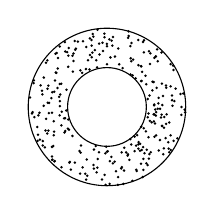
\begin{tikzpicture}[scale=0.5]
		% circles and line
		\draw (0,0) circle (1);
		\draw (0,0) circle (2);
		%\draw (0,0) -- (2,2);
		%\node[thick] at (0,0) {\pgfuseplotmark{o}};
		%markings fro interval
		%\draw[thick] (0.8,0.8) -- (1.6,1.6);
		%\node[rotate=45, thick] at (0.8,0.8) {\pgfuseplotmark{|}};
		%\node[rotate=45, thick] at (1.6,1.6) {\pgfuseplotmark{|}};
		%\node[thick] at (1.2,1.2) {\pgfuseplotmark{*}};
		% labels
		%\node at (1.0,1.4) {$r_\tau$};
		%				\node at (1.3,0) {$r_0$};
		%				\node at (2.3,0) {$r_1$};
		% random points
		\foreach \x in {1,...,300}{
			\pgfmathsetmacro{\r}{sqrt(random(100,400)/100)}%
			\pgfmathsetmacro{\a}{random(0,360)}%
			\pgfmathsetmacro{\x}{\r*sin(\a)}
			\pgfmathsetmacro{\y}{\r*cos(\a)}
			\node[fill,circle,inner sep=0pt,minimum size=1pt] at (\x ,\y) {};
		}
	\end{tikzpicture}
	\end{center}
	\scriptsize
	\begin{multline*}
		\ln{\pZ{n}{Q}} = - n^2 I_Q[\mu_Q]  + \frac{1}{2} n \ln n + \frac{n}{2} 	\left(\ln(2\pi) - 2 - E_Q[\mu_Q]\right) + \frac{1}{2} \ln(n) + \frac{\ln(2\pi)}{2}  + F_V[A_{[r_0, r_1]}] + \Boh(n^{-1}).
	\end{multline*}
	\begin{multline*}
		\!\!\!\!\!\!\!\!\!\!\! \ln{\pZ{n}{Q}} = - n^2 I_Q[\mu_Q]  + \frac{1}{2} n \ln n + \frac{n}{2} 	\left(\ln(2\pi) - 2 - E_Q[\mu_Q]\right) - \frac{5}{12} \ln (n) + \frac{\ln(2\pi)}{2} + \zeta'(-1) + F_V[D_{r_1}] + \Boh(n^{-1/12}(\ln n)^3).
	\end{multline*}
	\normalsize
	\begin{center}
		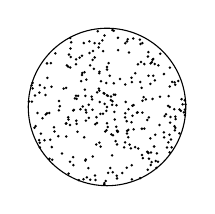
\begin{tikzpicture}[scale=0.5]
			% circles and line
			\draw (0,0) circle (2);
			%\draw (0,0) -- (2,2);
			%\node[thick] at (0,0) {\pgfuseplotmark{o}};
			%markings fro interval
			%\draw[thick] (0.0,0.0) -- (0.8,0.8);
			%\node[rotate=45, thick] at (0.8,0.8) {\pgfuseplotmark{|}};
			%\node[thick] at (0.3,0.3) {\pgfuseplotmark{*}};
			% labels
			%\node at (0.05,0.5) {$r_\tau$};
			%				\node at (-0.3,0) {$r_0$};
			%				\node at (2.3,0) {$r_1$};
			%\node at (1.0,0.6) {$r_\tau^*$};
			% random points
			\foreach \x in {1,...,300}{
				\pgfmathsetmacro{\r}{sqrt(random(0,400)/100)}%
				\pgfmathsetmacro{\a}{random(0,360)}%
				\pgfmathsetmacro{\x}{\r*sin(\a)}
				\pgfmathsetmacro{\y}{\r*cos(\a)}
				\node[fill,circle,inner sep=0pt,minimum size=1pt] at (\x ,\y) {};
			}
		\end{tikzpicture}
	\end{center}
	for the disk
	}
\end{frame}

